% 曲率：球面 K>0 与鞍面 K<0
\documentclass[border=4pt]{standalone}
\usepackage{tikz}
\usetikzlibrary{arrows.meta}
\usepackage{amsmath,amssymb}
\definecolor{fillA}{rgb}{0.45,0.45,0.45}
\definecolor{fillB}{rgb}{0.72,0.72,0.72}
\begin{document}
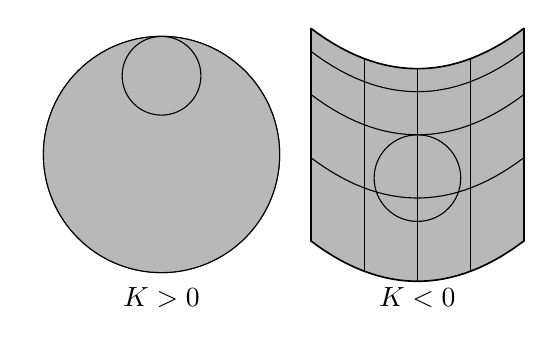
\begin{tikzpicture}[>=Stealth, line cap=round]
% ---------- 左：正曲率（球面） ----------
\draw (1.75,1.9) circle (1.5);
\fill[fillB] (1.116,3.26) arc (115:15:1.5) arc (15:-110:1.5) arc (-110:-245:1.5) -- cycle;
\draw (1.116,3.26) arc (115:15:1.5);
\draw (3.199,2.288) arc (15:-110:1.5);
\draw (1.237,0.4905) arc (-110:-245:1.5);
% 密切圆（与曲面同侧）
\draw (1.75,2.9) circle (0.5);
\node at (1.75,0.08) {$K>0$};
% ---------- 右：负曲率（鞍面） ----------
\fill[fillB]
  plot[domain=-1.35:1.35, samples=30] ({3.65}, {2.15+\x-0.28*\x*\x+0.5103})
  -- plot[domain=-1.35:1.35, samples=30] ({5.0+\x}, {2.15+0.28*\x*\x+0.8397})
  -- plot[domain=1.35:-1.35, samples=30] ({6.35}, {2.15+\x-0.28*\x*\x+0.5103})
  -- plot[domain=1.35:-1.35, samples=30] ({5.0+\x}, {2.15+0.28*\x*\x-1.8603})
  -- cycle;
\draw[semithick] plot[domain=-1.35:1.35, samples=30] ({3.65}, {2.15+\x-0.28*\x*\x+0.5103});
\draw[semithick] plot[domain=-1.35:1.35, samples=30] ({5.0+\x}, {2.15+0.28*\x*\x+0.8397});
\draw[semithick] plot[domain=1.35:-1.35, samples=30] ({6.35}, {2.15+\x-0.28*\x*\x+0.5103});
\draw[semithick] plot[domain=1.35:-1.35, samples=30] ({5.0+\x}, {2.15+0.28*\x*\x-1.8603});
\foreach \px in {-0.675,0,0.675}
  \draw plot[domain=-1.35:1.35, samples=30] ({5.0+\px}, {2.15+\x-0.28*\x*\x+0.28*\px*\px});
\foreach \py in {-0.675,0,0.675}
  \draw plot[domain=-1.35:1.35, samples=30] ({5.0+\x}, {2.15+0.28*\x*\x+\py-0.28*\py*\py});
% 密切圆（位于曲面另一侧）
\draw (5.0,1.6) circle (0.55);
\node at (5.0,0.08) {$K<0$};
\end{tikzpicture}
\end{document}
